\documentclass[a4paper,11pt,lualatex,ja=standard]{bxjsarticle}

% 数式
\usepackage{amsmath,amsfonts}
\usepackage{bm}
% 画像
\usepackage{graphicx}
% url
\usepackage{hyperref}

% ===== cover command =====
\newcommand{\cover}[3]{
  \thispagestyle{empty}
  \vspace*{4cm}
  \begin{center}
    {\LARGE #1}\\[2cm]
    {\Large #2}\\[3cm]
    {\large 氏名：#3}\\[1cm]
    % {\large 学籍番号：s2510063}
  \end{center}
  \newpage
}
% =========================

\begin{document}

% ===== cover =====
\cover{Perceptron Train Hole in Middle}{SyLab}{小林智輝}
% =================

\title{レポートタイトル}
\author{氏名}
\date{\today}

\section{Perceptron Train Hole in Middle}
\begin{verbatim}
  Watch a perceptron learn in real time on a "hole in the middle" 
  pattern: positive points surround one negative center point. 
  The classic perceptron update rule still applies 
  (only misclassified points trigger updates, with no weight decay), 
  but this shape is not linearly separable by a single line. 
  Reach 88.9% accuracy to reveal the flag.
\end{verbatim}

\begin{figure}[h]
  \centering
  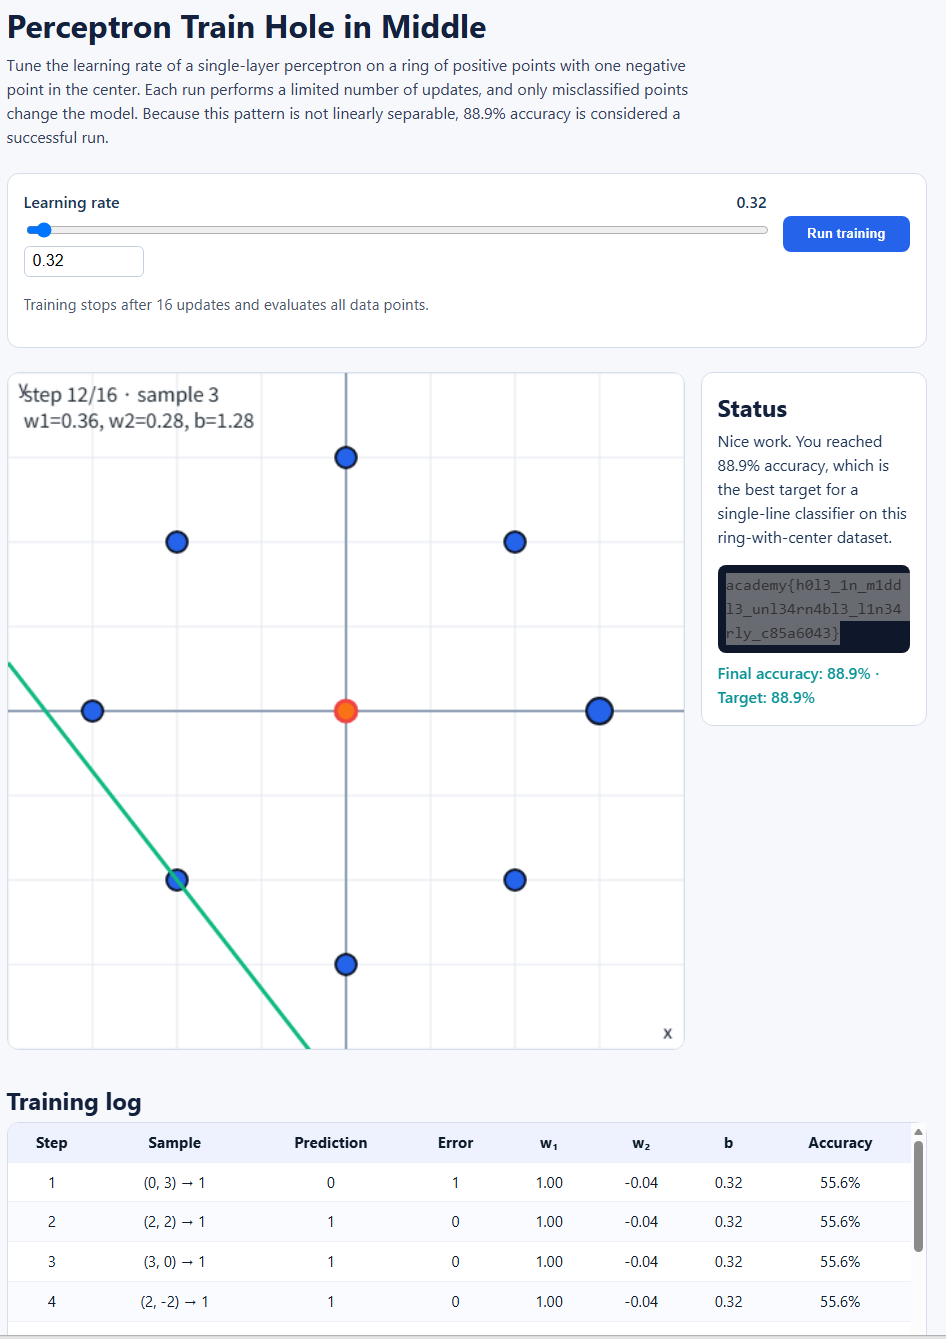
\includegraphics[width=0.7\linewidth]{03.png}
  \caption{img}
\end{figure}


\end{document}